\documentclass[a4paper,12pt]{article}
\usepackage[utf8]{inputenc}
\usepackage{graphicx}
\usepackage{multicolumn}
\usepackage{multirow}
\usepackage{booktabs}
\usepackage[indent=0pt,skip=3mm]{parskip}
\usepackage{array}
\usepackage{commath} % for abs ||
\usepackage{listings}             % Include the listings-package
\usepackage{tabs}
% \usepackage{colortbl}
\usepackage{url}
\usepackage{datetime}
\usepackage[ top=5cm, left=2cm, right=2cm, headheight=4cm]{geometry}
\usepackage{lastpage} % include last page numbering
\usepackage{fancyhdr}
\usepackage[table]{xcolor}% ctan.org/pkg/xcolor %FOR COLORS
% \usepackage{frame}
\settimeformat{ampmtime}
\setdefaultdate{\ddmmyyyydate}
\hyphenation{matriz}
\graphicspath{{figures/}{./images/}}
\newcommand{\eq}[1]{$#1$}
\newcommand{\head}[1]{{\bfseries #1}}
\newcommand{\header}[2][\tiny]{{\bfseries #1 #2}}

%%%%%%%%%%%%%%%%%%%%%%%%%%%%%%%%%%%%%%%%%%%%%%%%%%%%%%%%%%%%%%%%%%%%%%
%%%%%%%%%%%%%%%%%%%%%%%%%%%%%%%%%%%%%%%%%
\newsavebox{\mytabularheader}
\newsavebox{\mytabularheadertitle}
\setlength{\extrarowheight}{0.1cm}
%----------------------------------------------------------------------------------
%-----------------------------------------------------------------------------------------------
\sbox{\mytabularheadertitle}{%
  \begin{minipage}{.52\textwidth}
    \begin{center}
        \bfseries \scriptsize  UNIVERSIDAD NACIONAL DE SAN AGUSTIN\\
        FACULTAD DE INGENIERÍA DE PRODUCCIÓN Y SERVICIOS\\
        ESCUELA PROFESIONAL DE INGENIERÍA DE SISTEMA\\[3mm]
    \end{center}
  \end{minipage}
}

\sbox{\mytabularheader}{%
    \begin{minipage}{\textwidth}
        \centering
        \begin{tabular}{cp{8cm}c}
            
\includegraphics[scale=0.3]{epis_logo.png} & 
            \usebox{\mytabularheadertitle} &
            
\includegraphics[scale=0.05]{abet_logo.png} \\
            % \hline
            \multicolumn{3}{c}{Formato: Guía de Práctica de Laboratorio / Talleres / Centros de Simulación}\\
             &\multicolumn{1}{c}{Aprobación:  2022/03/01 Código: GUIA-PRLE-001} &  \\
        \end{tabular}
    \end{minipage}
}
%---------------------------------------
\renewcommand{\headrulewidth}{0pt}
\fancypagestyle{plain}{%
  \fancyhf{}%
  \fancyhf[ch]{\usebox{\mytabularheader}}
}
%--------------------------------------
\pagestyle{plain}
%%%%%%%%%%%%%%%%%%%%%%%%%%%%%%%%%%%%%%%%%%%%%%%%%%%%%%%%%%%%%%%%%%%%%%%%%%%%%%%%%%%%%%%%%%
\definecolor{blackRed}{cmyk}{0,81,76,31}

\begin{document}    
\lstset{language=Python,frame=single, firstnumber=1,basicstyle=\footnotesize,
numbers=left,showspaces=false,showstringspaces=false}   
    \begin{table}[t]
        \centering
        \begin{tabular}{|p{2.3cm}<{:}|m{1.7cm}|m{2.4cm}|m{2cm}|m{3cm}|m{0.6cm}|}
            \multicolumn{6}{c}{\cellcolor{red}{\leavevmode\color{white}\header{INFORMACIÓN BÁSICA}}}\\
            \hline
            \header{ASIGNATURA} & \multicolumn{5}{c}{\header[\footnotesize]{Física Computacional.}}\\
            \hline
            \header{\mbox{TÍTULO DE LA} PRÁCTICA} & \multicolumn{5}{c}{\header[\footnotesize]{Práctica de Ecuación diferencial de Laplace.}}\\
            \hline
            \header{\mbox{NÚMERO DE} PRÁCTICA} & {\header[\footnotesize]{05}} & \header{AÑO LECTIVO:} & {\header[\footnotesize]{2022-A}} & \header{NRO. SEMESTRE:} & \header[\footnotesize]{VII}\\
            \hline
            \header{\mbox{FECHA DE} \mbox{PRESENTACIÓN}} & \header{\today} & \header{HORA DE \mbox{PRESENTACIÓN:}} & \multicolumn{3}{c}{\header[\footnotesize]{\currenttime}}\\
            \hline
            \multicolumn{4}{l}{\header[\footnotesize]{Integrante(s): Alván Ventura Edsel Yael}} & \header{NOTA} & \\
            \hline
            \multicolumn{6}{l}{\header[\footnotesize]{DOCENTE(s):} \header[\footnotesize]{Danny Giancarlo Apaza Veliz.}} \\  
            \bottomrule
        \end{tabular}
    \end{table}
    \title{Práctica 6\\Física Computacional}
    \date{\vspace{-5ex}}
    \maketitle
    \begin{center}
        Escrito por\\
        Alván Ventura, Edsel Yael\\ \texttt{ealvan@unsa.edu.pe}
        \\[3mm]
        Profesor\\Apaza Veliz, Danny Giancarlo\\ \texttt{dapazav@unsa.edu.pe}\\[3mm]
        \today
    \end{center}
    % \newgeometry{top=2cm}
    \enlargethispage{\baselineskip}
    % \newpage
    \section{Problema 1}
    Implementar un código para la ecuación 15 de las diapositivas.
    
    \lstinputlisting[label=Archivo heatEquation.py]{heatEquation.py}
    
    \subsection{Resultados}
    El resultado de la implementación anterior es:
    \begin{figure}[h]
        \centering
        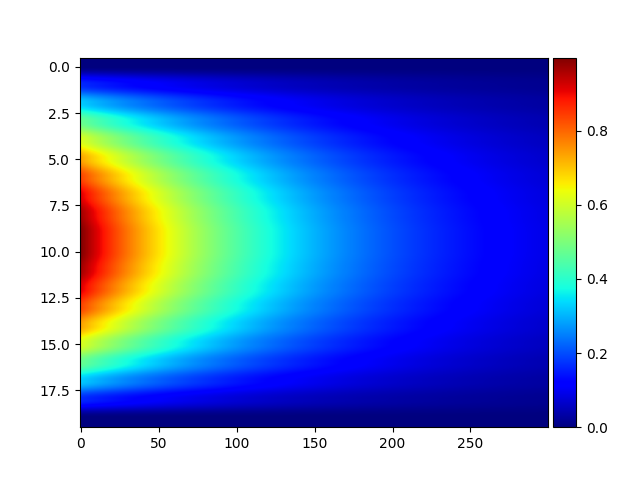
\includegraphics[width=0.8\textwidth]{ejer1_graph.png}
    \end{figure}

    \section{Problema 2}
    Modifique el código anterior de manera que permitan resolver problemas con condiciones en la frontera de la forma \eq{u(0,t) = g1(t) = 1} y \eq{u(a,t) = g2(t) = -1}.
    \subsection{Resolución}
    A continuación se muestra la implementación modificada para considerar las condiciones frontera:
    \lstinputlisting[label=Archivo heatEq.py]{heatEq.py}
    \begin{figure}[h]
        \centering
        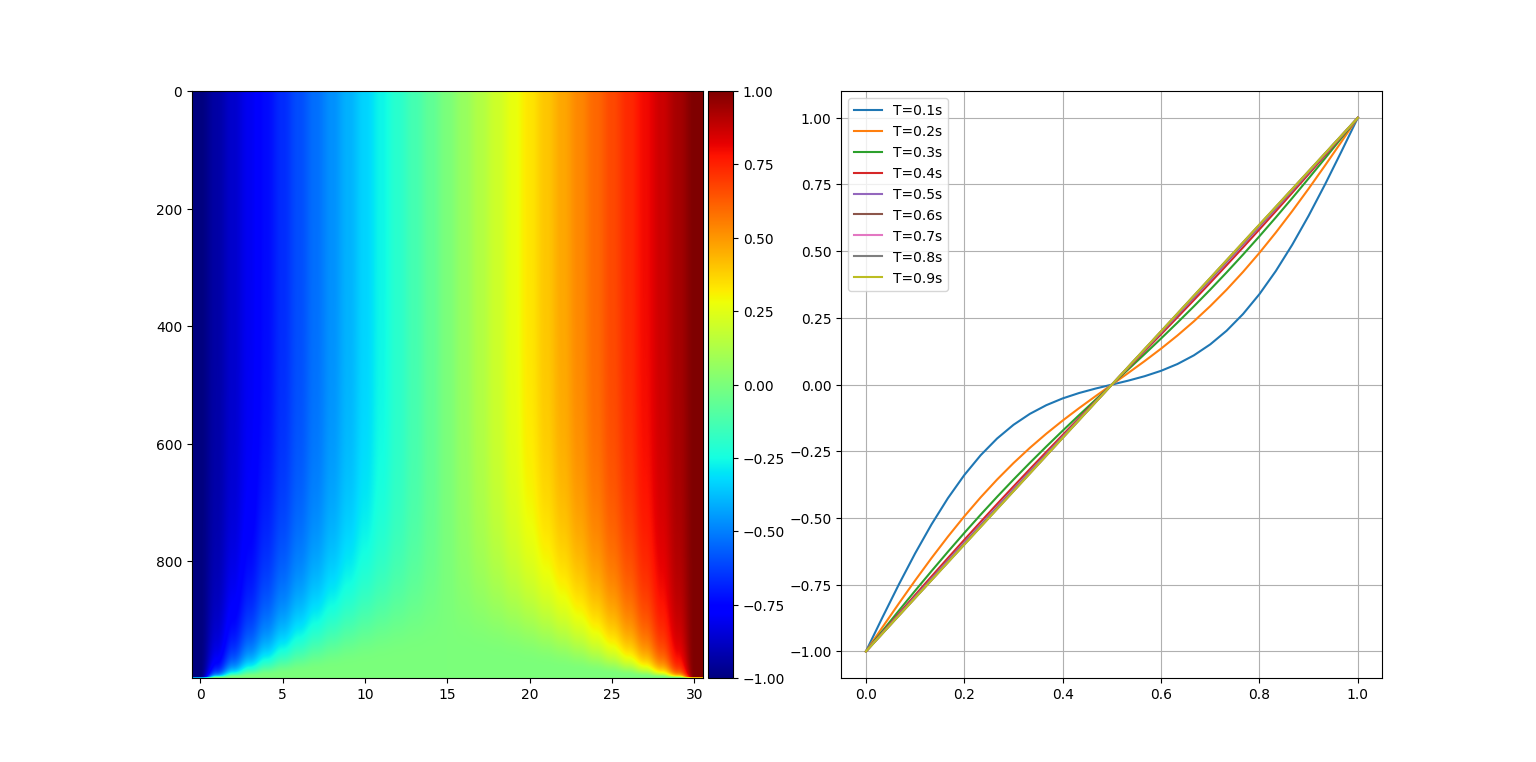
\includegraphics[width=0.8\textwidth]{ejer2_graph.png}
    \end{figure}
    
    \section{Problema 3}
    Sea \eq{f(x) = sen(n\pi x) + sen(n + 1)\pi x}, busque valores de h y k para que
    tenga una solución estable y varié n para ver comportamiento diferentes
    en las condiciones iniciales.

    \section{Problema 4}
    Sea \eq{f(x) = 4 - \abs{4x-1} - \abs{4x-3}}, busque valores de h y k para tener
    una solución estable.

\end{document}
